\documentclass[14pt,a4paper]{article}

\usepackage{fullpage}
\usepackage[utf8]{inputenc}
\usepackage{lmodern}
\usepackage{amsmath}
\usepackage{amssymb}
\usepackage{amsfonts}
\usepackage{pgfplots}
\usepackage{tikz}
\usepackage{pgf}

\begin{document}
%start
$
f''(x) = ${\large $ \frac{ \left( 6 - x \right)' x^3 -  \left( 6 - x \right) \left( x^3 \right) ' }{ \left(x^3 \right) ^2} $ } \\\\ $ = ${\large $ \frac{-1 * x^3 - \left(6-x\right) 3x^2}{x^6} $ } $ = ${\large $\frac{x^2[-x-\left(6-x\right)*3]}{x^6}$} \\\\ $ = ${\large $\frac{2x-18}{x^4} $ } \\\\ $ f''(x) = 0 $ \quad für $ x = 9 $ \\\\
$ I_4 = (- \infty, 0 ) : f''(-1)=-20 < 0 $ \\\\ $
I_5 = (0,9) : f''(1) = -16 < 0 $ \\\\ $
I_6 = (9, \infty) : f''(10) = $ {\large $\frac{2}{10^4}$ }$ = 2 * 10^{-4} > 0 $ \\\\ $ 
f''(x) < 0 $\quad $\forall y \in I_4 \Rightarrow f $ ist konkav in $ I_4 $ \\\\ $ f''(x)<0 $\quad$ \forall x \in I_5 \Rightarrow f $ ist konkav in $ I_5 $ \\\\ $  f''(x) > 0 $\quad$ \forall x \in I_6 \Rightarrow f $ ist konvex in $ I_6 $ \\\\ 
\underline{Extremwerte} \\\\ 
Bez.: Eine Stelle $ x_0 $ mit $ f'(x_0) = 0 $ heißt statioaer. \\
Satz: Sei $ f $ eine in $ [a,b] $ stetige und in $ (a,b) $ stetig diffenzierbare Funktion.\\
Dann gilt für eine Stelle $ x_0 \in (a,b) $ ein lokalen Minimums (oder lokalen Maximums) stets $ f'(x_0) = 0$.\\\\
\textit{Kriterium} : 
Sei $f$ eine in $(a,b) $ zweimal stetig differenzierbare Funktion mit $ f'(x_0) = 0$ . \\
$\left(x_0 \in (a,b)\right) $\\ a) Ist $ f''(x_0) <0$ ,so ist $ x_0 $ Stelle eines lokalen Maximums. \\ b)
Ist $ f''(x_0)$, so ist $ x_0 $ Stelle eines lokalen Minimums. \\ c)
$ n=2 m$ gerade, $f'(x_0)=f''(x_0)=f'''(x_0)=f^{n-1}(x_0) = 0, f^{(n)}(x_0) \neq 0 \Rightarrow $ relatives Extremum in $ x_0 $ \\ $ f^{(n)} (x_0) > 0 $ relatives Minimum \\$ f^{(n)}(x_0) $ relatives Maximum \\\\
Beispiel \\ $ f(x) = x^2, D_f = [-1,2] $ \\ $
f'(x) = 2x , x_0 = 0 $ \\ $
f''(x) = 2 > 0 $ \\\\
1) $ f'(0) = 0, f''(0) = 2 > 0
\Rightarrow x_0 = 0  $ ist Stelle eines lokalen Minimums \\\\
2) \\
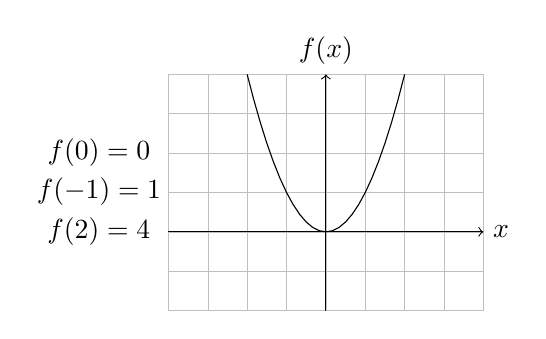
\begin{tikzpicture}[scale=0.5]
\draw[very thin,color=lightgray] (-4,-2) grid (4,4);
    \draw[->] (-4,0) -- (4,0) node[right] {$x$};
    \draw[->] (0,-2) -- (0,4) node[above] {$f(x)$};
    \draw node [left=82pt,above=20pt] {$f(0)=0 $};
    \draw node [left=82pt,above=6pt] {$f(-1) = 1$};
    \draw node [left=60pt] {$f(2) = 4$};
    \draw [color=black,domain=-2:2,] plot (\x,{pow(\x,2)});
\end{tikzpicture}
\\\\
$x_0$ ist auch Stelle eines globalen Minimums \\ 
$x_1 = 2$ ist Stelle eines globalen Maximums
\\ 
%stop
\end{document}